\documentclass[english,floatsintext,man]{apa6}

\usepackage{amssymb,amsmath}
\usepackage{ifxetex,ifluatex}
\usepackage{fixltx2e} % provides \textsubscript
\ifnum 0\ifxetex 1\fi\ifluatex 1\fi=0 % if pdftex
  \usepackage[T1]{fontenc}
  \usepackage[utf8]{inputenc}
\else % if luatex or xelatex
  \ifxetex
    \usepackage{mathspec}
    \usepackage{xltxtra,xunicode}
  \else
    \usepackage{fontspec}
  \fi
  \defaultfontfeatures{Mapping=tex-text,Scale=MatchLowercase}
  \newcommand{\euro}{€}
\fi
% use upquote if available, for straight quotes in verbatim environments
\IfFileExists{upquote.sty}{\usepackage{upquote}}{}
% use microtype if available
\IfFileExists{microtype.sty}{\usepackage{microtype}}{}

% Table formatting
\usepackage{longtable, booktabs}
\usepackage{lscape}
% \usepackage[counterclockwise]{rotating}   % Landscape page setup for large tables
\usepackage{multirow}		% Table styling
\usepackage{tabularx}		% Control Column width
\usepackage[flushleft]{threeparttable}	% Allows for three part tables with a specified notes section
\usepackage{threeparttablex}            % Lets threeparttable work with longtable

% Create new environments so endfloat can handle them
% \newenvironment{ltable}
%   {\begin{landscape}\begin{center}\begin{threeparttable}}
%   {\end{threeparttable}\end{center}\end{landscape}}

\newenvironment{lltable}
  {\begin{landscape}\begin{center}\begin{ThreePartTable}}
  {\end{ThreePartTable}\end{center}\end{landscape}}




% The following enables adjusting longtable caption width to table width
% Solution found at http://golatex.de/longtable-mit-caption-so-breit-wie-die-tabelle-t15767.html
\makeatletter
\newcommand\LastLTentrywidth{1em}
\newlength\longtablewidth
\setlength{\longtablewidth}{1in}
\newcommand\getlongtablewidth{%
 \begingroup
  \ifcsname LT@\roman{LT@tables}\endcsname
  \global\longtablewidth=0pt
  \renewcommand\LT@entry[2]{\global\advance\longtablewidth by ##2\relax\gdef\LastLTentrywidth{##2}}%
  \@nameuse{LT@\roman{LT@tables}}%
  \fi
\endgroup}


\ifxetex
  \usepackage[setpagesize=false, % page size defined by xetex
              unicode=false, % unicode breaks when used with xetex
              xetex]{hyperref}
\else
  \usepackage[unicode=true]{hyperref}
\fi
\hypersetup{breaklinks=true,
            pdfauthor={},
            pdftitle={XXX},
            colorlinks=true,
            citecolor=blue,
            urlcolor=blue,
            linkcolor=black,
            pdfborder={0 0 0}}
\urlstyle{same}  % don't use monospace font for urls

\setlength{\parindent}{0pt}
%\setlength{\parskip}{0pt plus 0pt minus 0pt}

\setlength{\emergencystretch}{3em}  % prevent overfull lines

\ifxetex
  \usepackage{polyglossia}
  \setmainlanguage{}
\else
  \usepackage[english]{babel}
\fi

% Manuscript styling
\captionsetup{font=singlespacing,justification=justified}
\usepackage{csquotes}
\usepackage{upgreek}



\usepackage{tikz} % Variable definition to generate author note

% fix for \tightlist problem in pandoc 1.14
\providecommand{\tightlist}{%
  \setlength{\itemsep}{0pt}\setlength{\parskip}{0pt}}

% Essential manuscript parts
  \title{XXX}

  \shorttitle{XXX}


  \author{XXX\textsuperscript{1}}

  \def\affdep{{""}}%
  \def\affcity{{""}}%

  \affiliation{
    \vspace{0.5cm}
          \textsuperscript{1} XXX  }

 % If no author_note is defined give only author information if available
      \newcounter{author}
                              \authornote{
            Correspondence concerning this article should be addressed to XXX, XXX. E-mail: XXX
          }
                    
  \note{XXX}

  \abstract{XXX}
  \keywords{XXX, XXX, XXX \\

    \indent Word count: X
  }





\usepackage{amsthm}
\newtheorem{theorem}{Theorem}
\newtheorem{lemma}{Lemma}
\theoremstyle{definition}
\newtheorem{definition}{Definition}
\newtheorem{corollary}{Corollary}
\newtheorem{proposition}{Proposition}
\theoremstyle{definition}
\newtheorem{example}{Example}
\theoremstyle{definition}
\newtheorem{exercise}{Exercise}
\theoremstyle{remark}
\newtheorem*{remark}{Remark}
\newtheorem*{solution}{Solution}
\begin{document}

\maketitle

\setcounter{secnumdepth}{0}



What is the relationship between student performance in language and
mathematics tasks? This is an important question that has been studied
extensively. For example, Abedi and Lord (2001) found that students
frequently feel anxiety in foreign language classes. XXX combined
several studies on language achievement and found that language-minority
students may need special treatment plans. Interestingly, language
appears to be related to performance in mathematics {[}XXX{]}. In one
study based on a survey of 1,174 8th grade students, XXX found that
students who were English language learners (ELLs) scored lower on math
tests than proficient speakers of English.

The purpose of the present research was to see if previous results
replicate in a new sample of language and mathematics learners. To test
this, we analysed data of student performance in Mathematics and
Portugese classes.

\section{Methods}\label{methods}

\subsection{Participants}\label{participants}

Data were collected from the UCI machine learning repository at
\url{http://archive.ics.uci.edu/ml/datasets/Student+Performance}. Data
from 395 students in a Mathematics class, and 2 students in a Portugese
class were collected.

\subsection{Procedure}\label{procedure}

The primary measures were three exam scores taken at the beginning,
middle, and end of each class.

\section{Results}\label{results}

Distributions of the three exam scores for the Mathematics and Portugese
classes are presented in Figure 1.

\begin{figure}

{\centering 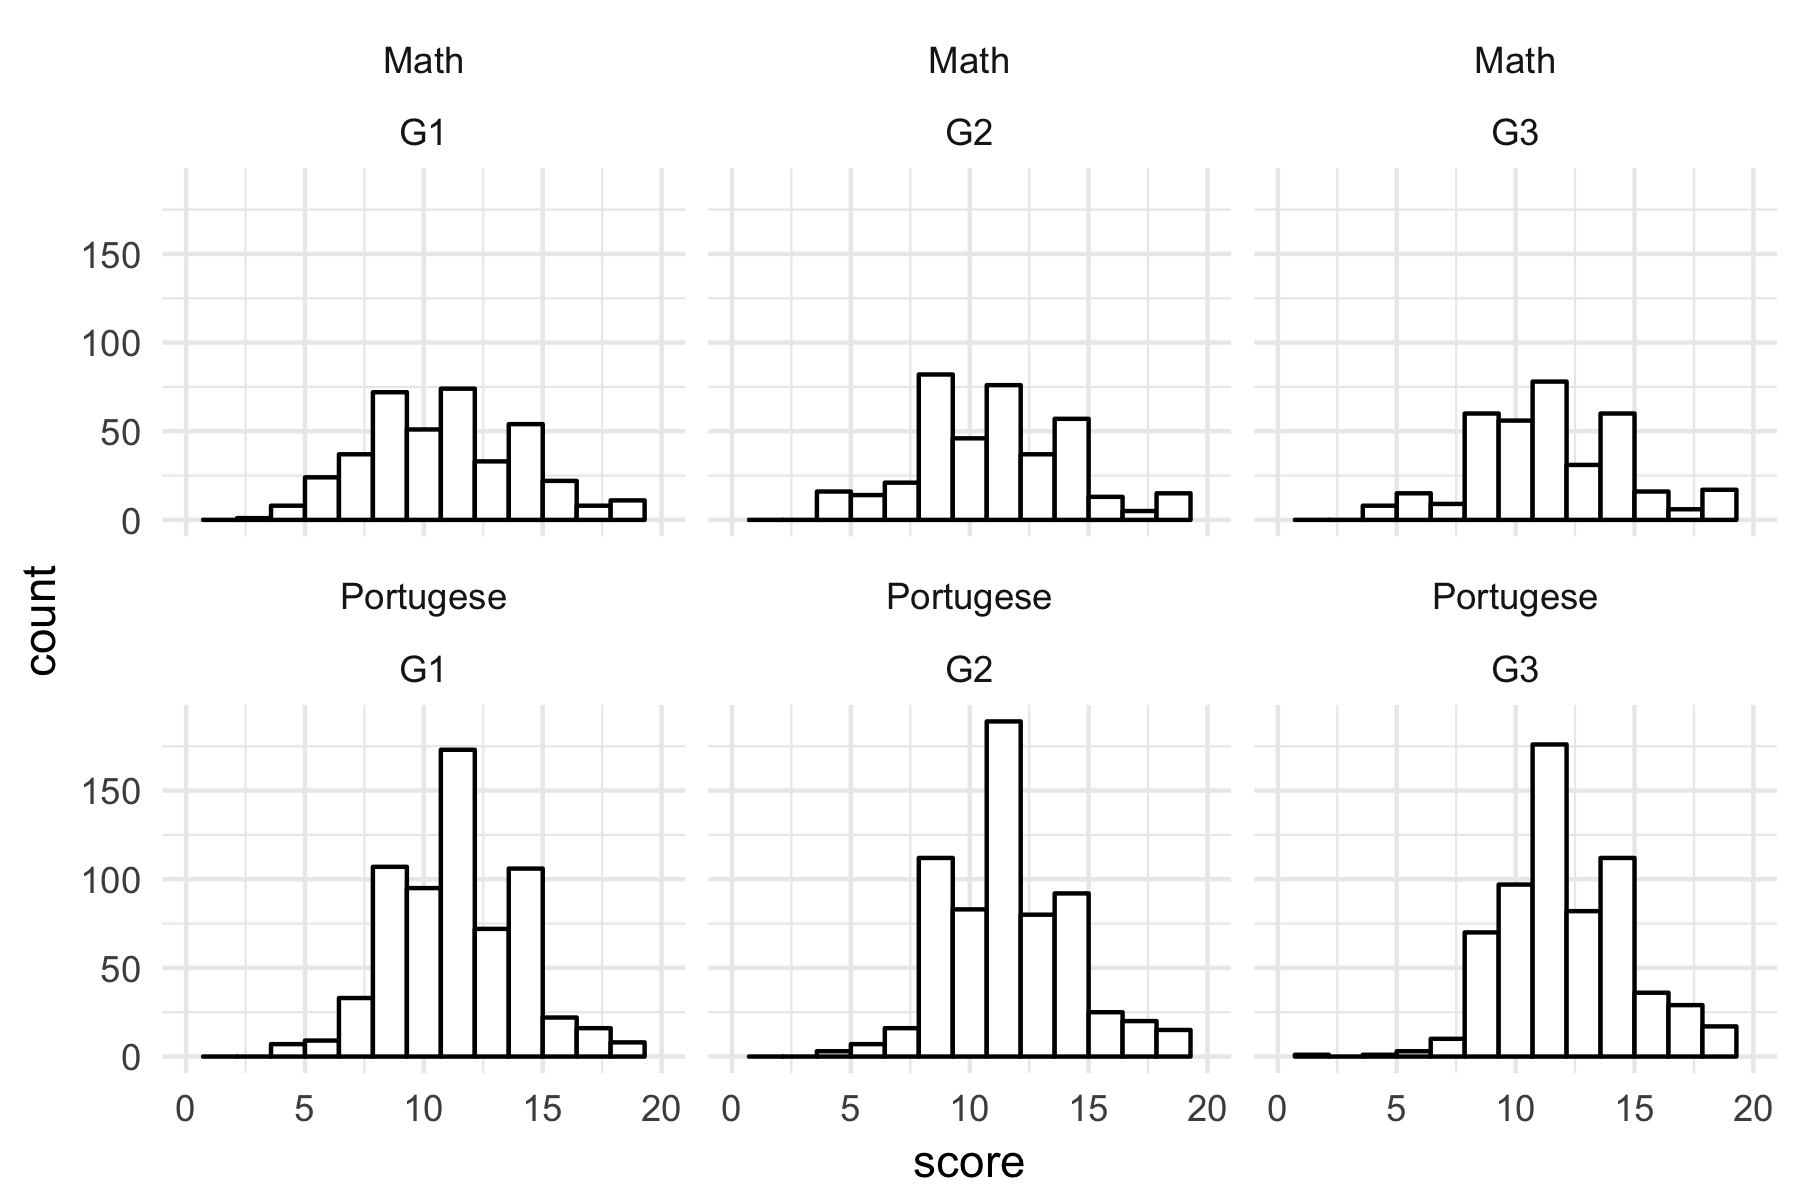
\includegraphics[width=1\linewidth]{studentAPA_files/figure-latex/fig1-1} 

}

\caption{XXX}\label{fig:fig1}
\end{figure}

Correlations between numeric predictors in the Math data are shown in
Figure X:

\begin{figure}

{\centering 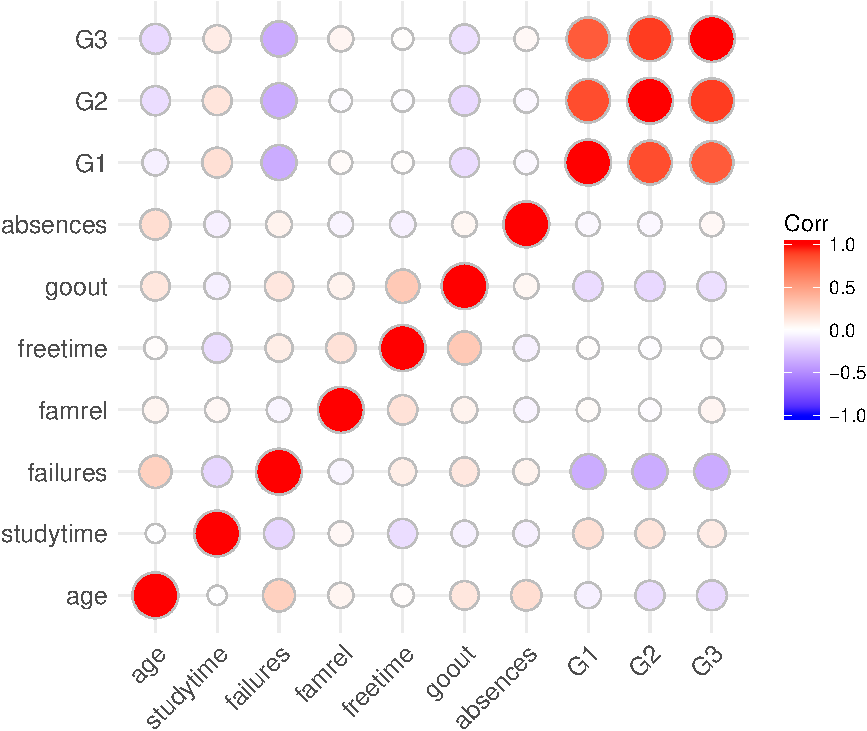
\includegraphics[width=0.7\linewidth]{studentAPA_files/figure-latex/fig2-1} 

}

\caption{XXX}\label{fig:fig2}
\end{figure}

Descriptive statistics of grades separated by sex and school are
presented in Tables 1 and 2. Grades tended to increase over the course
of the semester. For example, the mean grade in the first Portugese exam
was 2 which increased to 2 by the last exam.

Did men and women perform differently on the first exams in each class?
To tese this, we conducted two separate two-sample t-tests on first exam
scores as a function of sex. The t-test on Portugese exam 1 was
significant (t(589.90) = 2.69, p = 0.01), showing that women performed
better than men on the first Portugese exam.

The t-test on Math exam 1 was non-significant (t(2) = 2, p = 2), showing
no evidence for a difference between men and women on Math exam 1.

\section{Discussion}\label{discussion}

Understanding the relationship between language and math performance is
important for understanding learning. Our results are generally in line
with who found a relationship between language and mathematics
performance.

\section{References}\label{references}

\setlength{\parindent}{-0.5in} \setlength{\leftskip}{0.5in}
\setlength{\parskip}{8pt}

\hypertarget{refs}{}
\hypertarget{ref-abedi2001language}{}
Abedi, J., \& Lord, C. (2001). The language factor in mathematics tests.
\emph{Applied Measurement in Education}, \emph{14}(3), 219--234.






\end{document}
